\begin{figure}[htbp]
  \centering
  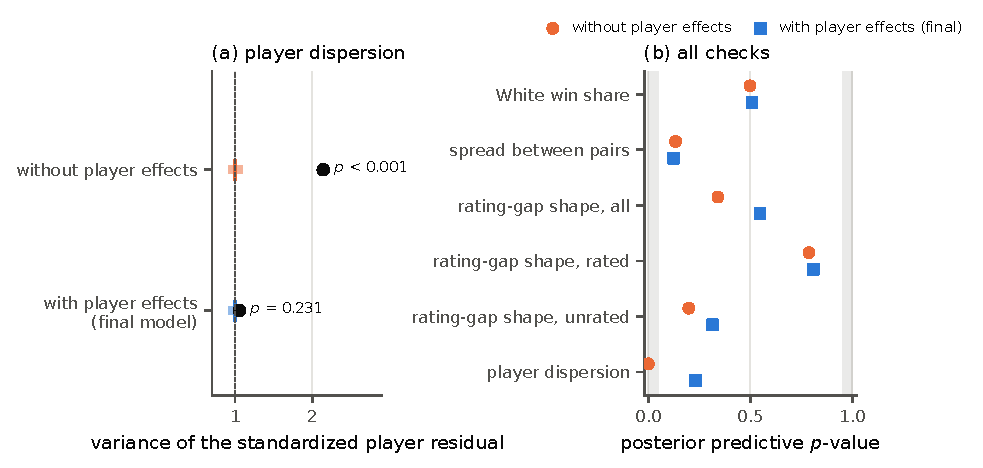
\includegraphics[width=\linewidth]{posterior_predictive_full.pdf}
  \caption{Posterior predictive checks of the final model (blue) and of the same model without player effects (orange), each from 4,000 data sets simulated from the posterior for the real games. (a): for each player with at least 10 games, the difference between their score and the score the model expects, divided by its standard deviation; the statistic is the variance of these standardized residuals over the players, close to 1 when a player's games are independent given the model. Black dots are the observed values averaged over posterior draws, bars the 90\% interval and ticks the median of the replicated values. Without player effects the observed dispersion is 2.14, far above what the model can produce (0.91 to 1.10): the same players keep beating, or missing, their rating. With player effects it is 1.06 against 0.91 to 1.10. (b): posterior predictive $p$-values of all the statistics, the share of replicated values at least as large as the observed one; values in the gray bands, below 0.05 or above 0.95, flag a feature of the data the model does not reproduce.}
  \label{fig:posterior_predictive_full}
\end{figure}
